
\chapter{2. Linear PDEs with matrix methods}

We start with a cliched example, the Poisson problem, because it is the right place to start.  Though the Poisson problem is a cliche in applied mathematics, it gives us the opportunity to use \PETSc for important tasks, including reading an unstructured mesh into \PETSc \pVec s, preallocation of a \pMat in parallel, and use of a linear solver (a \pKSP object) to solve large sparse systems.

\section{Example: The Poisson problem}

Let $\Omega \subset \RR^d$ be a bounded (open) region.  Suppose its boundary $\partial\Omega$ is well-behaved, for instance that it is Lipschitz-continuous \citep[section 1.2]{Ciarlet} or even polygonal.  Suppose $\partial\Omega$ is decomposed into (at least measurable) disjoint subsets $\partial_D \Omega$ and $\partial_N \Omega$ whose union is the entire boundary $\partial \Omega$.  The \emph{Poisson problem}, in strong form and including nonhomogeneous Dirichlet and Neumann boundary conditions, is\marginnote{%
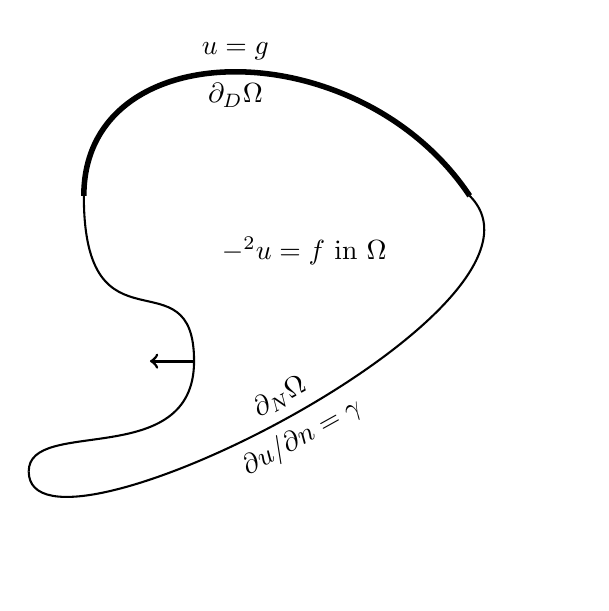
\begin{tikzpicture}[scale=0.7]
%\draw[gray,very thin] (-2,-6) grid (8,3);
\draw[line width=2pt] (0,0) .. controls (0,3) and (5,3) .. node[sloped,above] {$u=g$} node[sloped,below] {$\partial_D\Omega$} (7,0);
\draw[line width=0.75pt] (7,0) .. controls (9,-2) and (-1,-7) .. node[sloped,above] {$\partial_N\Omega$} node[sloped,below] {$\partial u/\partial n = \gamma$} (-1,-5);
\draw[line width=0.75pt] (-1,-5) .. controls (-1,-4) and (2,-5) .. (2,-3);
\draw[line width=0.75pt] (2,-3) .. controls (2,-1) and (0,-3) .. (0,0);
\draw[->,line width=1.0pt] (2,-3) -- (1.2,-3) node[below] {$\bn$}; % normal vector
\draw (4,-1) node {$- \grad^2 u = f$ in $\Omega$};
\end{tikzpicture}}
\begin{align}
- \grad^2 u &= f \quad \text{ on } \Omega, \label{poissonstrong} \\
u &= g \quad \text{ on } \partial_D \Omega, \notag \\
\frac{\partial u}{\partial n} &= \gamma \quad \text{ on } \partial_N \Omega \notag
\end{align}
where $\bn$ is the outward unit normal on $\partial \Omega$ and $\partial u/\partial n = \bn \cdot \grad u$.  The data of problem \eqref{poissonstrong}, besides the region $\Omega$ and its boundary, includes a \emph{source term} $f\in L^2(\Omega)$, \emph{Dirichlet data} $g\in L^2(\partial_N \Omega)$, and \emph{Neumann data} $\gamma\in L^2(\partial_N \Omega)$.

This Poisson problem models the distribution of temperature in a conducting object at steady state, the electrostatic potential, the equilibrium distribution from certain random walks, and many other other physical phenomena.  And it is linear, that is, if $u_1$ and $u_2$ are solutions then affine (i.e.~with coefficients that sum to one) linear combinations are also solutions.  More relevantly, it is a linear problem in the sense that finite-dimensional approximations of the Poisson problem are simply matrix problems.

As \eqref{poissonstrong} is stated there may be no solution where ``$\grad^2 u$'' makes sense as a continuous function, even for polygonal regions, continuous boundary values, and continuous source functions.  In particular, there may be no $u\in C^2(\Omega)$ which is continuous up to the boundary (i.e.~$u\in C(\bar\Omega)$) and so that $\grad^2 u = f$.  There is, however, a solution if we change to a \emph{weak formulation}.  Furthermore, if $\partial_D \Omega$ has positive size, in an appropriate sense \citep[Theorem 1.2.1]{Ciarlet}, then the solution of the weak formulation is unique.  We will state the weak formulation after defining function spaces.

Many mathematical concepts, including proofs that justify the above well-posedness claim, are covered in textbooks \citep{Ciarlet,Evans}.  These are technicalities for us, however.  Our goal is computational performance in cases where the Poisson problem is approximate-able without great effort, and mathematically well-behaved.  Indeed, in a moment we will restrict $\Omega$ to be the interior of a polygon. 

Recalling $L^2(\Omega)$ is the space of all square-integrable real functions on $\Omega$, define
    $$H^1(\Omega) = \{u\in L^2(\Omega) \big| \grad u \text{ exists a.e.~and } \grad u \in L^2(\Omega)\},$$
which is a Sobolev space \citep{Evans}.  This space has two subsets we will use, namely functions with value $g$ on $\partial_D \Omega$ and those with value $0$ on $\partial_D \Omega$, respectively, which we denote $H_g^1(\Omega)$ and $H_0^1(\Omega)$.  Note that $H_0^1(\Omega)$ is a linear subspace of $H^1(\Omega)$ while $H_g^1(\Omega)$ is generally not a subspace (e.g.~because the zero function is not in it).  Because $H_g^1(\Omega)$ is an affine subspace, from now on we refer to both $H_g^1(\Omega)$ and $H_0^1(\Omega)$ as ``subspaces''.

To get to the weak formulation of the Poisson problem we first suppose we already have a classical solution $u$ of \eqref{poissonstrong}.  Then we choose any $v\in H_0^1(\Omega)$, multiply the first equation in \eqref{poissonstrong} by $v$, and integrate by parts:
\begin{equation*}
\int_\Omega \grad u \cdot \grad v - \int_{\partial\Omega} \frac{\partial u}{\partial n} v = \int_\Omega f v.
\end{equation*}
Next\marginnote{%
{\color{red}Main ideas} of strong and weak formulations:\begin{itemize}
\item If $u \in H_g^1(\Omega)$ solves the strong form \eqref{poissonstrong} then it solves \eqref{poissonweak} also.
\item If $u \in H_g^1(\Omega)$ solves the weak form \eqref{poissonweak} then we accept it, by definition, as a solution of the Poisson problem.\end{itemize}} 
we use the other data, namely that $v=0$ on $\partial_D\Omega$ and that there is Neumann data $\gamma$ on $\partial_N\Omega$, in the above equation:
\begin{equation}
\int_\Omega \grad u \cdot \grad v = \int_\Omega f v + \int_{\partial_N\Omega} \gamma v\quad \text{ for any } v\in H_0^1(\Omega). \label{poissonweak}
\end{equation}

Equation \eqref{poissonweak} is the \emph{weak formulation} of the Poisson problem.  Any $u \in H_g^1(\Omega)$ satisfying \eqref{poissonweak} is called a \emph{weak solution}.  A key observation is that $u$ itself incorporates the Dirichlet boundary condition, because it lives in $H_g^1(\Omega)$, while both the Neumann boundary data $\gamma$ and the source function $f$ appear in equation \eqref{poissonweak}.


\section{A finite element method for the Poisson problem in the plane}

A \emph{finite element method} (FEM) for the Poisson problem comes from requiring the weak formulation \eqref{poissonweak} to be true for $u$ in a much smaller, indeed finite-dimensional, subspace of $H_g^1(\Omega)$.  Also $v$ will range over a finite-dimensional subspace of $H_0^1(\Omega)$.  In our case these subspaces will be essentially the same, so our method is a \emph{Galerkin} FEM.  We will build these finite-dimensional subspaces, in the current example, using an unstructured triangulation on $\Omega\subset \RR^2$.  In particular, from now on in this chapter we restrict to $d=2$ dimensions.

Furthermore, to make our finite-dimensional spaces true subspaces of $H^1(\Omega)$---to make our FEM \emph{conforming}---we also require that $\Omega$ be polygonal, with $\partial\Omega$ a closed polygon.  We require that the segments in $\partial\Omega$ each have positive length, and be either entirely in $\partial_D\Omega$ or entirely in $\partial_N\Omega$.  We also assume $\partial_D\Omega$ is a closed set so that, at vertices of the polygon $\partial \Omega$ where the Dirichlet boundary and Neumann boundary meet, the vertex itself is in the Dirichlet boundary.

\begin{marginfigure}
\input{samplepoly.1.tikz}
\caption{A triangulation $\Th$ with $K=22$ triangles (elements) numbered $k=0,1,\dots,K-1$ ({\color{red} red}) and $N=16$ nodes numbered $j=0,1,\dots,N-1$  ({\color{blue} blue}).  Nodes $\bx_0$, $\bx_1$, $\bx_2$, $\bx_3$ are in the Dirichlet boundary $\partial_D\Omega$.}
\label{fig:number-elements}
\end{marginfigure}

By definition, a \emph{triangulation} is a finite set of non-overlapping, non-empty open triangles $\triangle_k\subset \RR^2$ which tile $\Omega$:
\begin{equation*}
\Th = \left\{\triangle_k \quad\Big|\quad \cup_k \overline{\triangle}_k = \overline{\Omega} \quad \text{ and} \quad \Omega_k \cap \Omega_l = \emptyset \text{ if } k\ne l\right\}.
\end{equation*}
We index the $K$ triangles in $\Th$ by $k=0,\dots,K-1$.  An example is shown in Figure \ref{fig:number-elements}.  The subscript ``$h$'' in $\Th$ is, for now, just traditional.  It denotes the typical or maximum size $h$ (e.g.~diameter) of the triangles, and it serves as a reminder that we want to approximate the solution in the limit $h\to 0$.

The $N$ vertices (nodes) in the triangulation are indexed by $j=0,1,\dots,N-1$, as shown in the example in Figure \ref{fig:number-elements}.  Their planar locations are the geometric, as opposed to topological, information in a triangulation:
\begin{equation*}
\bx_j = (x_j,y_j).
\end{equation*}

In the above paragraphs the observant reader might note a contrast to \citet{Elmanetal2005}, which we generally follow, and many other references on the FEM or its implementation in languages like \Matlab.  Namely, our indexing is zero-based.  Indeed it is \emph{always} zero-based, as we implement in C and we want to avoid any confusion when comparing text and codes.  Not only are triangles and nodes numbered starting with zero, as above, but, breaking long mathematical traditions, even rows and columns of vectors and matrices will have numbering starting with zero.
 
We will informally call the triangles \emph{elements}, though there is more to the definition of ``element.''  We are going to approximate the Poisson problem with $\Pone$ finite elements, which means that our finite-dimensional subspace contains only piecewise-linear functions which are linear on each triangle $\triangle_k$.

For each node $j$ there is a $\Pone$ basis function, or ``hat'' function, $\phi_j(x,y)$ which is linear on each triangle, continuous on all of $\overline{\Omega}$, and equal to one on only one node $j$:\marginnote{%
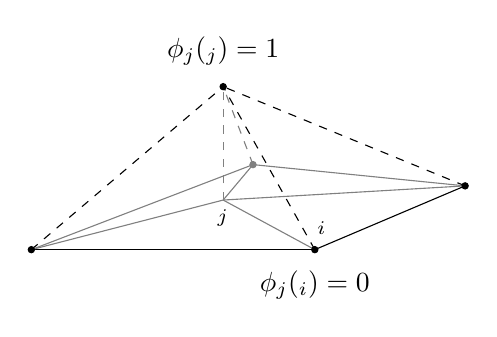
\begin{tikzpicture}[scale=0.9, z={(.707,.3)}]
    % (2,2,1) is top
    \draw[style=dashed] (0,0,0) -- (2,2,1); % to top from left
    \draw[style=dashed] (4,0,0) -- (2,2,1); %   ...  from front
    \draw[style=dashed] (4,0,3) -- (2,2,1); %   ...  from right
    \draw[color=gray, style=dashed] (0.3,0,4) -- (2,2,1); % from back
    \draw[color=gray, style=dashed] (2,0.4,1) -- (2,2,1); % from middle
    % draw base
    \draw (0,0,0) -- (4,0,0);
    \draw (4,0,0) -- (4,0,3);
    \draw[color=gray] (0,0,0) -- (0.3,0,4);
    \draw[color=gray] (0.3,0,4) -- (4,0,3);
    \draw[color=gray] (0,0,0) -- (2,0.4,1);
    \draw[color=gray] (2,0.4,1) -- (4,0,3);
    \draw[color=gray] (4,0,0) -- (2,0.4,1);
    \draw[color=gray] (2,0.4,1) -- (0.3,0,4);
    % draw \phi_j at nodes
    \filldraw (2,2,1) circle (1.25pt);
    \draw (2,2.5,1) node {$\phi_j(\bx_j)=1$};
    \draw (2,0.15,1) node {$\bx_j$};
    \filldraw (0,0,0) circle (1.25pt);
    \filldraw (4,0,0) circle (1.25pt);
    \draw (4,-0.5,0) node {$\phi_j(\bx_i)=0$};
    \draw (4.1,0.3,0) node {$\bx_i$};
    \filldraw (4,0,3) circle (1.25pt);
    \filldraw[color=gray] (0.3,0,4) circle (1.25pt);
\end{tikzpicture}
}%
\begin{equation*}
\phi_j(\bx_i) = \delta_{ij}.
\end{equation*}
The functions $\phi_j$ are in $H^1(\Omega)$, with piecewise-constant partial derivatives $\partial\phi_j/\partial x$ and $\partial\phi_j/\partial y$.  Also, the set $\{\phi_j\}_{j=0,\dots,N-1}$ is linearly-independent.  On each triangle, $\phi_j$ has three degrees of freedom.  That is, on $\triangle_k$ there exist coefficients $A_k,B_k,C_k\in\RR$ so that
\begin{equation*}
\phi_j(x,y) = A_k + B_k x + C_k y \quad \text{ on } \triangle_k.
\end{equation*}

We can immediately use these basis functions to approximate the Dirichlet data $g$ and ``extend'' it to the region $\Omega$.  We will assume from now on that the Dirichlet boundary $\partial_D\Omega$ is closed.  Then we index the $L$ nodes which are in the Dirichlet boundary, $\bx_{j_l} \in \partial_D\Omega$ for $l=0,\dots,L-1$.  (Figure \ref{fig:number-elements} shows an example with $L=4$ and $j_l=l$ for $l=0,1,2,3$, but a general index is allowed as long as the index values $j_l$ are well-defined.)  Now we can define an extended interpolant $\hat g$ of $g$ as the function which has the correct value on the Dirichlet boundary nodes and which extends to all of $\Omega$ in a continuous and piecewise-linear way:
\begin{equation}
\hat g(x,y) = \sum_{l=0,\dots,L} g(\bx_{j_l}) \phi_{j_l}(x,y). \label{hatgdefine}
\end{equation}

By using $\hat g$ and the basis functions $\phi_j$, we can now describe three finite-dimensional subspaces of $H^1(\Omega)$:\sidenote{Traditionally, basis functions for $S_g^h$ are called the \emph{trial} functions, and basis functions for $S_0^h$ are called \emph{test} functions.  We will generally just use the labels ``$S_g^h$'' and ``$S_0^h$.''}
\begin{align*}
S^h &= \Span\{\phi_j \,\big|\, \text{ all } j\,\}, \\
S_0^h &= \Span\{\phi_j \,\big|\, \bx_j \notin \partial_D \Omega\} \subset S^h, \\
S_g^h &= S_0^h + \hat g \subset S^h.
\end{align*}
Then $\dim(S^h)=N$ while $\dim(S_0^h)=\dim(S_g^h)=N-L$, with $S_g^h$ now clearly defined as an affine subspace of $S^h$.

Finally, our finite element method requires that the weak formulation  \eqref{poissonweak} be true of $u_h\in S_g^h$ for all $v\in S_0^h$.  Thus we first write $u_h$ in the basis for $S_g^h$ using $N-L$ unknown coefficients $u_j$:
\begin{equation}
u_h(x,y) = \hat g(x,y) + \sum_{\bx_j \notin \partial_D \Omega} u_j\, \phi_j(x,y). \label{uhexpand}
\end{equation}
Then we require that the weak formulation hold for all $\phi_i$ in the basis of $S_0^h$.  That is, using definition \eqref{hatgdefine} and expansion \eqref{uhexpand}, we require
\begin{align}
\sum_{j\big|\bx_j \notin \partial_D \Omega} u_j \int_\Omega \grad \phi_j \cdot \grad \phi_i &= \int_\Omega f \phi_i + \int_{\partial_N\Omega} \gamma \phi_i \label{poissonfem} \\
&\qquad - \sum_{l=0,\dots,L} g(\bx_{j_l})  \int_\Omega \grad \phi_{j_l} \cdot \grad \phi_i \notag
\end{align}
for all $i$ such that $\bx_i \notin \partial_D \Omega$.  The coefficients $u_j$, for all $j$ such that $\bx_j \notin \partial_D \Omega$, are the unknowns in this equation.

Note that the support (i.e.~nonzero set) of $\phi_j$ includes only the node $\bx_j$ and all triangles (elements) $\triangle_k$ for which $\bx_j$ is a node of $\triangle_k$.  Thus the integral ``$\int_\Omega \grad \phi_j \cdot \grad \phi_i$'' in \eqref{poissonfem} is often zero.  Specifically, it is zero if nodes $\bx_i$ and $\bx_j$ are not connected by an edge in the triangulation, equivalently if $\bx_i$ and $\bx_j$ are not both nodes of at least one triangle in the triangulation.



\section{Getting a triangular mesh into \PETSc}

We now take a break from mathematical constructions to do something practical with \PETSc.  While \PETSc itself does not include any tools for triangulating regions of the plane, we use the widely-available and easy-to-use \Triangle software \citep{Shewchuk1996} for this task.\sidenote{See \href{http://www.cs.cmu.edu/~quake/triangle.html}{www.cs.cmu.edu/$\sim$quake/ triangle.html} for documentation and source code of \Triangle. You can build it from source, but it is probably available as a package in your operating system.}  \Triangle, which is both limited to planar regions and only capable of writing ASCII files, is not a choice for performance.  It is convenient.

\Triangle uses a simply-formatted ASCII file (extension \texttt{.poly}) as input to describe a polygonal region $\Omega$ and to indicate the Dirichlet and Neumann portions of $\partial \Omega$.  For example, consider the input file \texttt{bump.poly} shown in Figure \ref{code:bumppoly}. 

\inputfromline{../c/bump.poly}{bump.poly}{A description of the boundary polygon in Figure \ref{fig:triangulation}, suitable for reading by \Triangle.}{16}{code:bumppoly}

This example polygon, a rectangle with a triangular bump in the base, is shown in Figure \ref{fig:bump-poly}.  It will reappear several times in these notes as we solve more and more interesting PDEs on it.  Note that the two extra vertices introduced along the bottom are used to identify that part of the boundary as Neumann.  (Recall, in this context, that the Dirichlet boundary is closed.)

\begin{marginfigure}
\input{bump.poly.tikz}
\caption{The polygon described by \texttt{bump.poly} in Figure \ref{code:bumppoly}.  The bold part is the Dirichlet boundary.  The lower boundary is Neumann, and has ``extra'' nodes to identify it as such.}
\label{fig:bump-poly}
\end{marginfigure}

The triangulation shown in Figure \ref{fig:triangulation} came from a single command which asks \Triangle to take \texttt{bump.poly} and generate a triangulation which is quality-checked \citep{Shewchuk1996} (option \texttt{-q}), which has triangles with maximum area of $1.0$ (option \texttt{-a1.0}), and including a polygon output file (option \texttt{-p}):
\begin{verbatim}
  $ triangle -pqa1.0 bump
\end{verbatim}
This command generates three ASCII files, \texttt{bump.1.poly}, \texttt{bump.1.node}, and  \texttt{bump.1.ele}.  These files define the new (i.e.~refined relative to \texttt{bump.poly}) polygonal boundary, the nodes locations, and the elements of the triangulation, respectively.  For example, \texttt{bump.1.node} has the numbering and node locations shown in blue in Figure \ref{fig:triangulation}.  The \Triangle software includes a minimal visualization tool which shows the triangulation graphically, and so
\begin{verbatim}
  $ showme bump
\end{verbatim}
will let the reader see both the boundary polygon in \texttt{bump.poly} and the triangulation in \texttt{bump.1.\{node,ele,poly\}}.

\begin{figure*}
% created by script tri2tikz.py command line:
%   ./tri2tikz.py --labelnodes --scale 2.0 --labeloffset 0.25 bump.1 bump.1.tikz
%
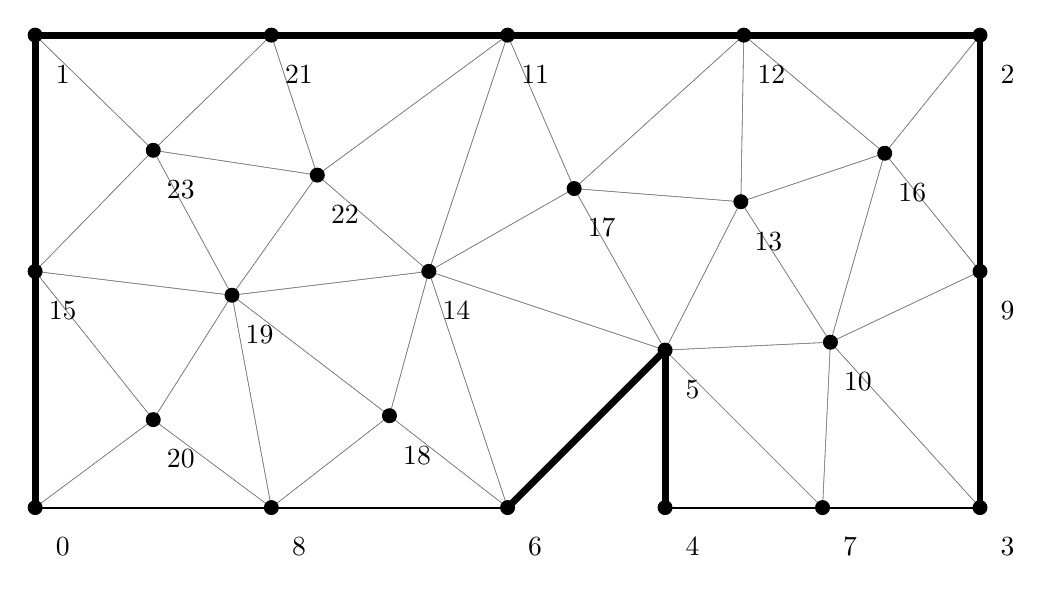
\begin{tikzpicture}[scale=2.000000]
  \draw[gray,very thin] (-1.500000,0.000000) -- (-2.250000,0.558372);
  \draw[gray,very thin] (-2.250000,0.558372) -- (-3.000000,0.000000);
  \draw[gray,very thin] (-3.000000,0.000000) -- (-1.500000,0.000000);
  \draw[gray,very thin] (-1.500000,0.000000) -- (0.000000,0.000000);
  \draw[gray,very thin] (0.000000,0.000000) -- (-0.750000,0.583333);
  \draw[gray,very thin] (-0.750000,0.583333) -- (-1.500000,0.000000);
  \draw[gray,very thin] (1.481325,1.942169) -- (0.422665,2.025778);
  \draw[gray,very thin] (0.422665,2.025778) -- (1.000000,1.000000);
  \draw[gray,very thin] (1.000000,1.000000) -- (1.481325,1.942169);
  \draw[gray,very thin] (-0.500000,1.500000) -- (0.000000,0.000000);
  \draw[gray,very thin] (0.000000,0.000000) -- (1.000000,1.000000);
  \draw[gray,very thin] (1.000000,1.000000) -- (-0.500000,1.500000);
  \draw[gray,very thin] (0.000000,3.000000) -- (-1.500000,3.000000);
  \draw[gray,very thin] (-1.500000,3.000000) -- (-1.208263,2.111158);
  \draw[gray,very thin] (-1.208263,2.111158) -- (0.000000,3.000000);
  \draw[gray,very thin] (2.000000,0.000000) -- (2.050000,1.050000);
  \draw[gray,very thin] (2.050000,1.050000) -- (1.000000,1.000000);
  \draw[gray,very thin] (1.000000,1.000000) -- (2.000000,0.000000);
  \draw[gray,very thin] (1.000000,0.000000) -- (2.000000,0.000000);
  \draw[gray,very thin] (2.000000,0.000000) -- (1.000000,1.000000);
  \draw[gray,very thin] (1.000000,1.000000) -- (1.000000,0.000000);
  \draw[gray,very thin] (2.394659,2.250000) -- (3.000000,1.500000);
  \draw[gray,very thin] (3.000000,1.500000) -- (3.000000,3.000000);
  \draw[gray,very thin] (3.000000,3.000000) -- (2.394659,2.250000);
  \draw[gray,very thin] (1.500000,3.000000) -- (0.422665,2.025778);
  \draw[gray,very thin] (0.422665,2.025778) -- (1.481325,1.942169);
  \draw[gray,very thin] (1.481325,1.942169) -- (1.500000,3.000000);
  \draw[gray,very thin] (2.050000,1.050000) -- (3.000000,0.000000);
  \draw[gray,very thin] (3.000000,0.000000) -- (3.000000,1.500000);
  \draw[gray,very thin] (3.000000,1.500000) -- (2.050000,1.050000);
  \draw[gray,very thin] (2.394659,2.250000) -- (2.050000,1.050000);
  \draw[gray,very thin] (2.050000,1.050000) -- (3.000000,1.500000);
  \draw[gray,very thin] (3.000000,1.500000) -- (2.394659,2.250000);
  \draw[gray,very thin] (-1.500000,3.000000) -- (-3.000000,3.000000);
  \draw[gray,very thin] (-3.000000,3.000000) -- (-2.250000,2.268853);
  \draw[gray,very thin] (-2.250000,2.268853) -- (-1.500000,3.000000);
  \draw[gray,very thin] (1.481325,1.942169) -- (1.000000,1.000000);
  \draw[gray,very thin] (1.000000,1.000000) -- (2.050000,1.050000);
  \draw[gray,very thin] (2.050000,1.050000) -- (1.481325,1.942169);
  \draw[gray,very thin] (3.000000,0.000000) -- (2.050000,1.050000);
  \draw[gray,very thin] (2.050000,1.050000) -- (2.000000,0.000000);
  \draw[gray,very thin] (2.000000,0.000000) -- (3.000000,0.000000);
  \draw[gray,very thin] (0.422665,2.025778) -- (1.500000,3.000000);
  \draw[gray,very thin] (1.500000,3.000000) -- (0.000000,3.000000);
  \draw[gray,very thin] (0.000000,3.000000) -- (0.422665,2.025778);
  \draw[gray,very thin] (2.394659,2.250000) -- (1.500000,3.000000);
  \draw[gray,very thin] (1.500000,3.000000) -- (1.481325,1.942169);
  \draw[gray,very thin] (1.481325,1.942169) -- (2.394659,2.250000);
  \draw[gray,very thin] (-1.750000,1.348485) -- (-0.750000,0.583333);
  \draw[gray,very thin] (-0.750000,0.583333) -- (-0.500000,1.500000);
  \draw[gray,very thin] (-0.500000,1.500000) -- (-1.750000,1.348485);
  \draw[gray,very thin] (-1.500000,0.000000) -- (-0.750000,0.583333);
  \draw[gray,very thin] (-0.750000,0.583333) -- (-1.750000,1.348485);
  \draw[gray,very thin] (-1.750000,1.348485) -- (-1.500000,0.000000);
  \draw[gray,very thin] (1.500000,3.000000) -- (2.394659,2.250000);
  \draw[gray,very thin] (2.394659,2.250000) -- (3.000000,3.000000);
  \draw[gray,very thin] (3.000000,3.000000) -- (1.500000,3.000000);
  \draw[gray,very thin] (2.050000,1.050000) -- (2.394659,2.250000);
  \draw[gray,very thin] (2.394659,2.250000) -- (1.481325,1.942169);
  \draw[gray,very thin] (1.481325,1.942169) -- (2.050000,1.050000);
  \draw[gray,very thin] (0.000000,3.000000) -- (-0.500000,1.500000);
  \draw[gray,very thin] (-0.500000,1.500000) -- (0.422665,2.025778);
  \draw[gray,very thin] (0.422665,2.025778) -- (0.000000,3.000000);
  \draw[gray,very thin] (1.000000,1.000000) -- (0.422665,2.025778);
  \draw[gray,very thin] (0.422665,2.025778) -- (-0.500000,1.500000);
  \draw[gray,very thin] (-0.500000,1.500000) -- (1.000000,1.000000);
  \draw[gray,very thin] (0.000000,0.000000) -- (-0.500000,1.500000);
  \draw[gray,very thin] (-0.500000,1.500000) -- (-0.750000,0.583333);
  \draw[gray,very thin] (-0.750000,0.583333) -- (0.000000,0.000000);
  \draw[gray,very thin] (-1.750000,1.348485) -- (-2.250000,2.268853);
  \draw[gray,very thin] (-2.250000,2.268853) -- (-3.000000,1.500000);
  \draw[gray,very thin] (-3.000000,1.500000) -- (-1.750000,1.348485);
  \draw[gray,very thin] (-3.000000,1.500000) -- (-3.000000,0.000000);
  \draw[gray,very thin] (-3.000000,0.000000) -- (-2.250000,0.558372);
  \draw[gray,very thin] (-2.250000,0.558372) -- (-3.000000,1.500000);
  \draw[gray,very thin] (-1.500000,0.000000) -- (-1.750000,1.348485);
  \draw[gray,very thin] (-1.750000,1.348485) -- (-2.250000,0.558372);
  \draw[gray,very thin] (-2.250000,0.558372) -- (-1.500000,0.000000);
  \draw[gray,very thin] (-3.000000,1.500000) -- (-2.250000,0.558372);
  \draw[gray,very thin] (-2.250000,0.558372) -- (-1.750000,1.348485);
  \draw[gray,very thin] (-1.750000,1.348485) -- (-3.000000,1.500000);
  \draw[gray,very thin] (0.000000,3.000000) -- (-1.208263,2.111158);
  \draw[gray,very thin] (-1.208263,2.111158) -- (-0.500000,1.500000);
  \draw[gray,very thin] (-0.500000,1.500000) -- (0.000000,3.000000);
  \draw[gray,very thin] (-0.500000,1.500000) -- (-1.208263,2.111158);
  \draw[gray,very thin] (-1.208263,2.111158) -- (-1.750000,1.348485);
  \draw[gray,very thin] (-1.750000,1.348485) -- (-0.500000,1.500000);
  \draw[gray,very thin] (-2.250000,2.268853) -- (-1.208263,2.111158);
  \draw[gray,very thin] (-1.208263,2.111158) -- (-1.500000,3.000000);
  \draw[gray,very thin] (-1.500000,3.000000) -- (-2.250000,2.268853);
  \draw[gray,very thin] (-3.000000,1.500000) -- (-2.250000,2.268853);
  \draw[gray,very thin] (-2.250000,2.268853) -- (-3.000000,3.000000);
  \draw[gray,very thin] (-3.000000,3.000000) -- (-3.000000,1.500000);
  \draw[gray,very thin] (-1.208263,2.111158) -- (-2.250000,2.268853);
  \draw[gray,very thin] (-2.250000,2.268853) -- (-1.750000,1.348485);
  \draw[gray,very thin] (-1.750000,1.348485) -- (-1.208263,2.111158);
  \draw[line width=2.5pt] (-3.000000,0.000000) -- (-3.000000,1.500000);
  \draw[line width=2.5pt] (-3.000000,3.000000) -- (-1.500000,3.000000);
  \draw[line width=2.5pt] (3.000000,3.000000) -- (3.000000,1.500000);
  \draw[line width=0.75pt] (3.000000,0.000000) -- (2.000000,0.000000);
  \draw[line width=0.75pt] (2.000000,0.000000) -- (1.000000,0.000000);
  \draw[line width=2.5pt] (1.000000,1.000000) -- (1.000000,0.000000);
  \draw[line width=2.5pt] (0.000000,0.000000) -- (1.000000,1.000000);
  \draw[line width=0.75pt] (0.000000,0.000000) -- (-1.500000,0.000000);
  \draw[line width=0.75pt] (-1.500000,0.000000) -- (-3.000000,0.000000);
  \draw[line width=2.5pt] (3.000000,1.500000) -- (3.000000,0.000000);
  \draw[line width=2.5pt] (0.000000,3.000000) -- (1.500000,3.000000);
  \draw[line width=2.5pt] (1.500000,3.000000) -- (3.000000,3.000000);
  \draw[line width=2.5pt] (-3.000000,1.500000) -- (-3.000000,3.000000);
  \draw[line width=2.5pt] (-1.500000,3.000000) -- (0.000000,3.000000);
  \draw (-2.825000,-0.250000) node {$0$};
  \filldraw (-3.000000,0.000000) circle (1.25pt);
  \draw (-2.825000,2.750000) node {$1$};
  \filldraw (-3.000000,3.000000) circle (1.25pt);
  \draw (3.175000,2.750000) node {$2$};
  \filldraw (3.000000,3.000000) circle (1.25pt);
  \draw (3.175000,-0.250000) node {$3$};
  \filldraw (3.000000,0.000000) circle (1.25pt);
  \draw (1.175000,-0.250000) node {$4$};
  \filldraw (1.000000,0.000000) circle (1.25pt);
  \draw (1.175000,0.750000) node {$5$};
  \filldraw (1.000000,1.000000) circle (1.25pt);
  \draw (0.175000,-0.250000) node {$6$};
  \filldraw (0.000000,0.000000) circle (1.25pt);
  \draw (2.175000,-0.250000) node {$7$};
  \filldraw (2.000000,0.000000) circle (1.25pt);
  \draw (-1.325000,-0.250000) node {$8$};
  \filldraw (-1.500000,0.000000) circle (1.25pt);
  \draw (3.175000,1.250000) node {$9$};
  \filldraw (3.000000,1.500000) circle (1.25pt);
  \draw (2.225000,0.800000) node {$10$};
  \filldraw (2.050000,1.050000) circle (1.25pt);
  \draw (0.175000,2.750000) node {$11$};
  \filldraw (0.000000,3.000000) circle (1.25pt);
  \draw (1.675000,2.750000) node {$12$};
  \filldraw (1.500000,3.000000) circle (1.25pt);
  \draw (1.656325,1.692169) node {$13$};
  \filldraw (1.481325,1.942169) circle (1.25pt);
  \draw (-0.325000,1.250000) node {$14$};
  \filldraw (-0.500000,1.500000) circle (1.25pt);
  \draw (-2.825000,1.250000) node {$15$};
  \filldraw (-3.000000,1.500000) circle (1.25pt);
  \draw (2.569659,2.000000) node {$16$};
  \filldraw (2.394659,2.250000) circle (1.25pt);
  \draw (0.597665,1.775778) node {$17$};
  \filldraw (0.422665,2.025778) circle (1.25pt);
  \draw (-0.575000,0.333333) node {$18$};
  \filldraw (-0.750000,0.583333) circle (1.25pt);
  \draw (-1.575000,1.098485) node {$19$};
  \filldraw (-1.750000,1.348485) circle (1.25pt);
  \draw (-2.075000,0.308372) node {$20$};
  \filldraw (-2.250000,0.558372) circle (1.25pt);
  \draw (-1.325000,2.750000) node {$21$};
  \filldraw (-1.500000,3.000000) circle (1.25pt);
  \draw (-1.033263,1.861158) node {$22$};
  \filldraw (-1.208263,2.111158) circle (1.25pt);
  \draw (-2.075000,2.018853) node {$23$};
  \filldraw (-2.250000,2.268853) circle (1.25pt);
\end{tikzpicture}

\caption{A FEM triangulation generated by \Triangle.  {\color{blue} Nodes} are labeled by $j=0,\dots,N-1$ with $N=24$ and {\color{red} elements} are labeled by $k=0,\dots,K-1$ with $K=32$.}
\label{fig:triangulation}
\end{figure*}

The ASCII files produced by \Triangle produces are not in a good format for large meshes.  On the one hand we will accept this, as a convenience needed for portability and readability, as we will mostly focus on the scalability of the solution process once the mesh is loaded.  On the other hand, we do demonstrate how files are read in parallel, but this is based on first doing a mundane and un-scalable task in \PETSc.  Namely we read the ASCII \Triangle files serially onto a single processor and write out a binary file in \PETSc format.  The binary file both describes the mesh element-by-element and can be read in parallel.  The code \texttt{c2convert.c} does the conversion.  It is invoked, for the present purposes, by
\begin{verbatim}
  $ c2convert -f bump.1
\end{verbatim}
This reads ASCII files \texttt{bump.1.\{node,ele,poly\}} and writes a \PETSc-formatted binary file \texttt{bump.1.petsc}.

We show \texttt{c2convert.c} in detail (Figure \ref{code:trianglepartone}).  It starts with a standard preamble which we will not show for future codes.  Here \PETSc is initialized and we get the rank of the current (MPI) process.  Then we use the pair \texttt{PetscOptions\{Begin,End\}} to bracket the reading of the two options we need, namely a string containing the filename root, and a flag which determines whether \texttt{c2convert.c} will read back its \texttt{.petsc} output as a check.  This \texttt{Begin}/\texttt{End} pair allows \PETSc to give a helpful message, which describes the options for various components including the application code, when we run ``\texttt{c2convert -h}''.

\cinputpart{c2convert.c}{The standard preamble, and determination of filenames using \PETSc option processing.}{I}{//STARTPREAMBLE}{//ENDFILENAME}{code:trianglepartone}

The next part of \texttt{c2convert.c} is in Figure \ref{code:triangleparttwo}.  Starting here we only ask the first process (``rank zero'') in the MPI communicator to do any work.\sidenote{This code can be invoked ``\texttt{mpiexec -n NN c2convert}'', but it behaves as a serial code, other than the ``\texttt{-check}'' part.}  This part of the code first reads the header information in the \texttt{.node} file, and allocates \PETSc \pVec s according.  We use \texttt{VecCreateSeq} to allocate the a sequential \pVec \texttt{vx}, which contains the $x$-coordinate of the nodes, only on the rank zero process.  Then \texttt{VecDuplicate} is used to allocate two more \pVec s with the same layout, \texttt{vy} and \texttt{vBT}.  This last \pVec will contain a flag $\{0,2,3\}$ for each node, where $0$ is an interior node, $2$ is a Dirichlet boundary node, and $3$ is a Neumann boundary node.

\cinputpart{c2convert.c}{Start reading ASCII files with the \textsc{triangle}-generated mesh: Go to rank zero processor, read node header, and allocate \pVec s accordingly.  Then read nodes.}{II}{//ENDFILENAME}{//ENDREADNODES}{code:triangleparttwo}

Then we read the node locations from the \texttt{.node} file.  The reading itself is done with the standard C library call \texttt{fscanf}.  Then \texttt{VecSetValues} is used to set one entry at a time.  After setting these values, which stores a list of entrys into an internal \PETSc dynamic data structure, we ask \PETSc to do the assembly.  Assembly of \pVec s and \pMat s is done so often that we put it in a C preprocessor macro (Figure \ref{code:convenience}).

\inputwhole{../c/convenience.h}{convenience.h}{Macros for assembly.}{code:convenience}

The next part of \texttt{c2convert.c} is in Figure \ref{code:trianglepartthree}.  This looks like the previous part: we read boundary polygon information from the \texttt{.poly} file.  Each segment of the boundary polygon corresponds to two node indices.  We store the segments in a \pVec with blocksize 2.

\cinputpart{c2convert.c}{On rank zero: Read polygon information.}{III}{//ENDREADNODES}{//ENDREADPOLYGONS}{code:trianglepartthree}

The next short part (Figure \ref{code:trianglepartfour}) reads the header information in the \texttt{.ele} file and allocates a \pVec called \texttt{vE} for the elements.  This part of the code is an important transformation of the data structures.  In fact, \texttt{vE} has block size 15,\marginnote{A \PETSc \pVec is designed to hold \texttt{PetscScalar} data types, i.e.~\texttt{double} in most cases.  So we are being quite wasteful for integer indices and boolean flags.} and, in contrast to the format from \Triangle, it contains all the information about each element that we need to do assemble the matrix equation.  Each of its blocks is the following C \texttt{struct}:
\newcommand*\FancyVerbStartString{//STARTSTRUCT}
\newcommand*\FancyVerbStopString{//ENDSTRUCT}
\VerbatimInput[fontfamily=courier,%
               fontsize=\small]{../c/readmesh.h}
\let\FancyVerbStartString\relax
\let\FancyVerbStopString\relax

\cinputpart{c2convert.c}{On rank zero: Read element header information and allocate a \pVec with block size 15.}{IV}{//ENDREADPOLYGONS}{//STARTREADELEMENTS}{code:trianglepartfour}

In the next part (Figure \ref{code:trianglepartfive}) we fill the \pVec for elements with all of the information read so far, including the node indices for each element which we read from the \texttt{.ele} file.  This stage is fundamentally serial, because we must look at the entire mesh to find the node coordinates and node/segment boundary type for each node and edge of each element.  In this part there is an important detail about triangulations, which affects the data structure for elements.  Namely, we cannot tell if an edge of an element is in the boundary just by whether both endpoints are in the boundary.  For example, the element (triangle) labeled ``5'' in Figure \ref{fig:triangulation} has an edge from node 5 (on the Dirichlet boundary) to node 7 (on the Neumann boundary).  But triangle 5 is \emph{not} a boundary element.  Thus we need to have list of flags for the boundary segments themselves.  Thus the \texttt{elementtype} structure above has both a boundary type for each node of each element and a boundary type for each edge of each element.

\cinputpart{c2convert.c}{On rank zero: Read node indices for each element and fill element data structure.}{V}{//STARTREADELEMENTS}{//ENDREADELEMENTS}{code:trianglepartfive}

At this point we have the whole triangulation into \PETSc \pVec s.  Now is the easy and last part of \texttt{c2convert.c}, shown in Figure \ref{code:trianglepartsix}.  We simply create a \PETSc ``viewer'' and ``view'' all of the \pVec s which contain the mesh.  We will be able to reread these \pVec s in parallel, as long as we re-read them in the same order.

\cinputpart{c2convert.c}{On rank zero: Write the mesh in \PETSc binary format.}{VI}{//ENDREADELEMENTS}{//ENDRANK0}{code:trianglepartsix}

To tell the truth, we have not shown the last part of \texttt{c2convert.c}.  That truly-final bit of code checks if option \texttt{-check} is given, and if so we read back the binary file in parallel.  This part of \texttt{c2convert.c} calls two methods from a re-used component \texttt{readmesh.c} which we do show.  The first is a method \texttt{getmeshfile()} which finds a \PETSc binary file from a \texttt{-f} option (Figure \ref{code:readmeshparttwo}).  The second method \texttt{readmesh()} creates and reads three \pVec s in parallel from it (Figure \ref{code:readmeshparttwo}).  Note that prefixes are set on each \pVec so that the block size is correctly read.

\cinputpart{readmesh.c}{Determine the filename of a \PETSc binary file that has a mesh.}{I}{//STARTGET}{//ENDGET}{code:readmeshpartone}

\cinputpart{readmesh.c}{Read the mesh in parallel from the file.}{II}{//STARTREADMESH}{//ENDREADMESH}{code:readmeshparttwo}


\section{Constructing the FEM linear system}

Now that we can get a triangulation into \PETSc, we can return to the finite-dimensional weak formulation \eqref{poissonfem}.  It is simply a matrix equation (linear system).  We will write a code, namely for matrix \emph{preallocation} and \emph{assembly}, which builds \PETSc \pMat and \pVec objects to contain this problem, and then we will use a \PETSc \pKSP object to solve it.

For ease of construction we include the node-wise Dirichlet conditions $u_j=g(\bx_j)$ as equations in this linear system, so that the matrix has $N$ columns and $N$ rows if there are $N$ nodes in total.  That is, we include a row and column for every node $\bx_j$ including $\bx_j\in\partial_D\Omega$.  Thus we define $A \in \RR^{N\times N}$ to have entries
\begin{equation*}
a_{ij} = \int_\Omega \grad \phi_j \cdot \grad \phi_i,
\end{equation*}
if $\bx_i \notin \partial_D \Omega$ and $\bx_j \notin \partial_D \Omega$.  Otherwise
\begin{equation*}
a_{ij} = \delta_{ij},
\end{equation*}
that is, if $\bx_i \in \partial_D \Omega$ or $\bx_j \in \partial_D \Omega$.  Because $j=0,1,\dots,N-1$, notice that we index rows and columns of matrices and vectors starting with zero.\sidenote{This follows C and \PETSc conventions, but is opposed to long-standing traditions about linear algebra!}

We can immediately observe that $A$ is \emph{symmetric} because $a_{ij}=a_{ji}$.  Furthermore it is \emph{sparse}, that is, most entries are zero, at least for triangulations with more than a handful of triangles.  These facts have profound consequences on the algorithms we will choose when solving our linear system
\begin{equation}
A \bu = \bb. \label{poissonmatrix}
\end{equation}

The right side of \eqref{poissonmatrix} also comes from \eqref{poissonfem}.  Define the vector $\bb\in\RR^N$ with entries
    $$b_i = \int_\Omega f \phi_i + \int_{\partial_N\Omega} \gamma \phi_i - \sum_{l=0,\dots,L} g(\bx_{j_l})  \int_\Omega \grad \phi_{j_l} \cdot \grad \phi_i$$
if $\bx_i \notin \partial_D \Omega$, while if $\bx_i \in \partial_D \Omega$ then
    $$b_i = g(\bx_{i}).$$

In practice we \emph{don't} initially build $A$ as described above.  We initially build a matrix $\tilde A$ which is the same size as $A$ but which ignors the boundary nodes and their type (i.e.~Dirichlet or Neumann).  All entries of $\tilde A$ are computed by the first formula above for $a_{ij}$, that is, the entries are
\begin{equation*}
\tilde a_{ij} = \int_\Omega \grad \phi_j \cdot \grad \phi_i
\end{equation*}
for all $i,j=0,1,\dots,N$.  Also we initially compute a simpler right-hand side $\tilde \bb\in\RR^N$ with entries
    $$\tilde b_i = \int_\Omega f \phi_i + \int_{\partial_N\Omega} \gamma \phi_i$$
if $\bx_i \notin \partial_D \Omega$, while if $\bx_i \in \partial_D \Omega$ then
    $$\tilde b_i = g(\bx_{i})$$
as before.

Note that the equation ``$\tilde A \bu =\tilde \bb$'' is \emph{not} equivalent to $A\bu = \bb$ because in the former linear system rows $i$ where $\bx_i \in \partial_D \Omega$ are nonsensical; the value $(\tilde A \bu)_i$ is not compatible with $\tilde \bb_i$.  Thus the next step is to  ``edit'' $\tilde A$ in each Dirichlet node row, that is, for each $i$ where $\bx_i \in \partial_D \Omega$, by replacing the whole row by the corresponding row of the identity.  Furthermore, in each column $j$ for which $\bx_j \in \partial_D \Omega$, we move all entries $\tilde a_{ij}$ where $i$ is \emph{not} a Dirichlet row index, over to the right-hand side, but multiplied by the negative of the boundary value $g(\bx_{j})$.  Informally we write
    $$\tilde b_i \to \tilde b_i - g(\bx_{j}) \tilde a_{ij}$$
for these transformations.  After the completion of this ``editing'' stage, for all Dirichlet rows and columns, we get $A$ and $\bb$.  Since this part of the matrix assembly is a key stage of understanding our FEM codes, we give a concrete example.

\medskip\noindent\hrulefill
\begin{example} In Figure \ref{fig:squarefour} there are five nodes.  The $i=1,2$ nodes live in the (closed) Dirichlet boundary $\partial_D \Omega$.  The matrix $\tilde A$ has this nonzero pattern; the zero entries are spaces:\begin{marginfigure}
\input{squarefour.tikz}
\caption{A triangulation of a square with five nodes.  The top segment is the Dirichlet boundary.}
\label{fig:squarefour}
\end{marginfigure}%
\begin{equation*}
\tilde A = \begin{bmatrix}
\X & \X &    & \X & \X \\
\X & \X & \X &    & \X \\
   & \X & \X & \X & \X \\
\X &    & \X & \X & \X \\
\X & \X & \X & \X & \X
\end{bmatrix}.
\end{equation*}
Note $\tilde a_{ij}=0$ only where the integral $\int_\Omega \grad \phi_j \cdot \grad \phi_i$ is zero, which is somewhat rare in this small (coarse)-mesh case.  Now we color the $i=1,2$ or $j=1,2$ entries which will be edited:\marginnote{{\color{red} Potential gotcha}:  The first row of any matrix in this book is numbered ``$0$.''  Likewise the first column.}
\begin{equation*}
\tilde A = \begin{bmatrix}
\X & \redX &    & \X & \X \\
\blueX & \blueX & \blueX &    & \blueX \\
   & \blueX & \blueX & \blueX & \blueX \\
\X &    & \redX & \X & \X \\
\X & \redX & \redX & \X & \X
\end{bmatrix}.
\end{equation*}
The {\color{blue} blue} entries are changed to $0$ or $1$ so that these rows become rows of the identity; their computed values are tossed out.  The {\color{red} red} entries, specifically the four entries $\tilde a_{01}$, $\tilde a_{32}$, $\tilde a_{41}$, and $\tilde a_{42}$, are moved over to the right side, however; their values get used.  Formulas for the $i=0,3,4$ entries of the final vector $\bb$ in terms of the initially-computed vector $\tilde\bb$ are:
\begin{align*}
b_0 &= \tilde b_0 - g(\bx_1) \tilde a_{01} \\
b_3 &= \tilde b_3 - g(\bx_2) \tilde a_{32} \\
b_4 &= \tilde b_4 - g(\bx_1) \tilde a_{41} - g(\bx_2) \tilde a_{42}.
\end{align*}
Note $b_1=\tilde b_1=g(\bx_1)$ and $b_2 = \tilde b_2 = g(\bx_2)$.  The final matrix $A$ has this pattern:
\begin{equation*}
A = \begin{bmatrix}
\X & & & \X & \X \\
 & \,1\, & & & \\
 & & \,1\, & & \\
\X & & & \X & \X \\
\X & & & \X & \X
\end{bmatrix}.
\end{equation*}
\end{example}
\noindent\hrulefill

\bigskip

Note that the initial construction is already correct in the case where $\partial_D \Omega$ is the empty set.  That is, in the Neumann-only case $A=\tilde A$ and $\bb = \tilde \bb$.  However, in this case $u=(\text{constant})$ solves $-\grad^2 u=0$ with $\partial u/\partial n = 0$ on the whole boundary $\partial_N \Omega = \partial \Omega$, so equation \eqref{poissonweak} only determines the solution up to an additive constant.  Because the Poisson problem does not have a unique solution, we will have to tell \PETSc about the extra constant solutions, the null space, to solve it.


\section{Assembling the matrix equation, element by element}

Each entry $\tilde a_{ij}$ of the initial matrix $\tilde A$ is not even computed in one step.  Rather, we compute contributions to these entries from each element.  Furthermore we do this in parallel because, from \texttt{readmesh.c} above, the \pVec called \texttt{E}, containing a list of elements of type \texttt{elementtype},\sidenote{Defined just before Figure \ref{code:trianglepartfour}.} is distributed across the processes.

To explain such element-by-element assembly we first define the integral over just one triangle $\triangle_k$, and we give it a code-style name:
    $$\text{\texttt{a(k,i,j)}} = \int_{\triangle_k} \grad \phi_j \cdot \grad \phi_i.$$
Note that
    $$\tilde a_{ij} = \sum_k \phantom{.}\text{\texttt{a(k,i,j)}}$$
with this notation.  If \texttt{E} denotes an array of \texttt{elementtype}, then for each triangle $\triangle_k$ we have a global node index for each of the three vertices.  That is, for each $k=0,1,\dots,K-1$ we have
    $$\text{\texttt{E[k].j[q]}} \in \{0,1,\dots,N-1\} \quad \text{ for } q = 0,1,2.$$
Now the element-by-element assembly of $\tilde A$ follows this pseudocode:
\begin{Verbatim}[fontsize=\small]
A = 0                           // N x N sparse matrix with entries a(i,j)
for k = 0 to K-1                // loop through all elements
    for q = 0 to 2
        i = E[k].j[q]           // row index
        for r = 0 to 2
            j = E[k].j[r]       // column index
            a(i,j) += a(k,i,j)  // add contribution from element k
\end{Verbatim}
\medskip\noindent
In the above pseudocode it would be natural to write
    $$\text{\texttt{a(k,q,r)}} = \text{\texttt{a(k,i,j)}},$$
because on a given triangle $\triangle_k$, the global indices $i,j$ are functions of the local node indices $q,r\in\{0,1,2\}$ on the triangle.  Now we need to both compute \texttt{a(k,q,r)} concretely and we need to implement the ``editing'' strategy which turns $\tilde A$ into $A$.

A standard approach to computing the element-wise integrals \texttt{a(k,q,r)} is to refer each triangle $\triangle_k$ to a reference triangle $\triangle_\ast$ with vertices $(0,0),\,(1,0),\,(0,1)$, as shown in Figure \ref{fig:isoparametric}.  The linear map from $\triangle_\ast$ to a generic triangle $\triangle$ with vertices $(x_0,y_0),\,(x_1,y_1),\,(x_2,y_2)$, as shown in the Figure, is
\begin{align}
x(\xi,\eta) &= x_0 + (x_1-x_0) \xi + (x_2-x_0) \eta, \label{trianglemap} \\
y(\xi,\eta) &= y_0 + (y_1-y_0) \xi + (y_2-y_0) \eta. \notag
\end{align}

\begin{marginfigure}
\begin{tikzpicture}[scale=1.1,
    decoration={
      markings,
      mark=at position 1 with {\arrow[scale=1.8,gray]{latex}};
    }]
% left x,y axes
    \draw[->, gray, very thin] (1.5,0) -- (4.0,0);
    \draw[->, gray, very thin] (2,-0.5) -- (2,2.4);
    \draw (4.1,-0.1) node {$x$};
    \draw (1.9,2.4) node {$y$};
    \filldraw (1.7,1) circle (1.25pt);    % (x_0,y_0)
    \filldraw (3.5,-0.3) circle (1.25pt); % (x_1,y_1)
    \filldraw (3.0,2.0) circle (1.25pt);  % (x_2,y_2)
    \draw (1.4,1.3) node {$(x_0,y_0)$};
    \draw (3.5,-0.6) node {$(x_1,y_1)$};
    \draw (3.0,2.3) node {$(x_2,y_2)$};
    \draw[line width=1pt] (1.7,1) -- (3.5,-0.3) -- (3.0,2.0) -- cycle;
    \draw (2.7,1.0) node {$\triangle$};
% right xi,eta axes
    \draw[->, gray, very thin] (4.6,0) -- (6.6,0);
    \draw[->, gray, very thin] (5,-0.4) -- (5,2.0);
    \draw (6.7,-0.1) node {$\xi$};
    \draw (4.9,2.05) node {$\eta$};
    \filldraw (5,0) circle (1.25pt);  % (0,0)
    \filldraw (6,0) circle (1.25pt);  % (1,0)
    \filldraw (5,1) circle (1.25pt);  % (0,1)
    \draw (5.3,-0.3) node {$(0,0)$};
    \draw (6.3,0.2) node {$(1,0)$};
    \draw (5.4,1.1) node {$(0,1)$};
    \draw[line width=1pt] (5,0) -- (6,0) -- (5,1) -- cycle;
    \draw (5.3,0.3) node {$\triangle_\ast$};
% arrows connecting nodes
    \draw[gray, postaction={decorate}] (5,0) -- (1.7,1.03);
    \draw[gray, postaction={decorate}] (6,0) -- (3.5,-0.3);
    \draw[gray, postaction={decorate}] (5,1) -- (3.0,2.0);
\end{tikzpicture}
\smallskip
\caption{Mapping of a generic triangle $\triangle$ from the reference triangle $\triangle_\ast$.}
\label{fig:isoparametric}
\end{marginfigure}

\noindent Furthermore, on $\triangle_\ast$ any linear function is a linear combination of these three local basis functions:
\begin{equation*}
\chi_0(\xi,\eta) = 1-\xi-\eta, \qquad \chi_1(\xi,\eta) = \xi, \qquad \chi_2(\xi,\eta) = \eta.
\end{equation*}
Using a local index $q=0,1,2$ for the vertices of $\triangle$, each of the basis functions $\phi_q$ is the mapped version of the corresponding $\chi_q$:
   $$\phi_q(x(\xi,\eta),y(\xi,\eta)) = \chi_q(\xi,\eta).$$
Through this last formula and the mapping \eqref{trianglemap} from the reference element one can check that
   $$\phi_q(x_r,y_r) = \chi_q(\xi_r,\eta_r) = \delta_{qr}$$
where we naturally define $(\xi_0,\eta_0)=(0,0)$, $(\xi_1,\eta_1)=(1,0)$, and $(\xi_2,\eta_2)=(0,1)$.

The Jacobian\sidenote{By definition, the \emph{Jacobian} of a smooth map $F$ is its linearization, so that if $\by=F(\bx)$ and if $\by+\Delta\by = F(\bx+\Delta\bx)$ then $\Delta \by = J(\bx) \Delta\bx + O(|\Delta\bx|^2)$.} of map \eqref{trianglemap} is
% CAUTION: Elman (1.37) uses "Jacobian" for the transpose of this, the true Jacobian (e.g. in Newton later)
\begin{equation}
J = \begin{bmatrix}
    \frac{\partial x}{\partial \xi} & \frac{\partial x}{\partial \eta} \\[0.2em]
    \frac{\partial y}{\partial \xi} & \frac{\partial y}{\partial \eta}
    \end{bmatrix}
    =
    \begin{bmatrix}
    x_1-x_0 & x_2-x_0 \\
    y_1-y_0 & y_2-y_0
    \end{bmatrix}.  \label{trianglejacobian}
\end{equation}
On the other hand, by the chain rule, we can make the silly calculation
\begin{equation*}
\begin{bmatrix}
    1 & 0 \\[0.2em]
    0 & 1
\end{bmatrix}
=\begin{bmatrix}
    \frac{\partial x}{\partial x} & \frac{\partial x}{\partial y} \\[0.2em]
    \frac{\partial y}{\partial x} & \frac{\partial y}{\partial y}
\end{bmatrix}
=
\begin{bmatrix}
    \frac{\partial x}{\partial \xi} & \frac{\partial x}{\partial \eta} \\[0.2em]
    \frac{\partial y}{\partial \xi} & \frac{\partial y}{\partial \eta}
\end{bmatrix}
\begin{bmatrix}
    \frac{\partial \xi}{\partial x} & \frac{\partial \xi}{\partial y} \\[0.2em]
    \frac{\partial \eta}{\partial x} & \frac{\partial \eta}{\partial y}
\end{bmatrix},
\end{equation*}
which is to say ``$I=J\; J^{-1}$.''  So, because we can invert the $2\times 2$ matrix $J$ by hand (e.g.~Cramer's rule),\sidenote{This is useful below because we need computable formulas for ``$\partial \xi/\partial x$'' and similar terms.}
\begin{equation*}
\begin{bmatrix}
    \frac{\partial \xi}{\partial x} & \frac{\partial \xi}{\partial y} \\[0.2em]
    \frac{\partial \eta}{\partial x} & \frac{\partial \eta}{\partial y}
\end{bmatrix}
= J^{-1}
= \frac{1}{\det(J)}
\begin{bmatrix}
    \frac{\partial y}{\partial \eta} & -\frac{\partial x}{\partial \eta} \\[0.2em]
    -\frac{\partial y}{\partial \xi} & \frac{\partial x}{\partial \xi}
\end{bmatrix}
= \frac{1}{\det(J)}
\begin{bmatrix}
    y_2-y_0 & x_0-x_2 \\
    y_0-y_1 & x_1-x_0
\end{bmatrix},
\end{equation*}
and also $\det(J) = (x_1-x_0)(y_2-y_0)-(y_1-y_0)(x_2-x_0)$.  It will be helpful to have shorthand for this, so based on these entries of $J^{-1}$, let $y_{20}=y_2-y_0$, $x_{02}=x_0-x_2$, $y_{01}=y_0-y_1$ and $x_{10}=x_1-x_0$ be the four differences we actually compute.  In terms of these differences,
\begin{equation}
\begin{bmatrix}
    \frac{\partial \xi}{\partial x} & \frac{\partial \xi}{\partial y} \\[0.2em]
    \frac{\partial \eta}{\partial x} & \frac{\partial \eta}{\partial y}
\end{bmatrix}
= \frac{1}{\det(J)}
\begin{bmatrix}
    y_{20} & x_{02} \\
    y_{01} & x_{10}
\end{bmatrix}
\quad \text{ and } \quad
\det(J) = x_{10} y_{20} - y_{01} x_{02}. \label{dxietadxy}
\end{equation}

In these terms, and recalling both the change-of-variables formula for integrals and the chain rule,
\begin{align}
\text{\texttt{a(k,q,r)}} &= \int_{\triangle} \grad\phi_q \cdot \grad\phi_r \label{elementcontrib} \\
   &= \int_{\triangle} \frac{\partial\phi_q}{\partial x} \frac{\partial\phi_r}{\partial x} + \frac{\partial\phi_q}{\partial y} \frac{\partial\phi_r}{\partial y} \; dx \, dy  \notag \\
   &= \int_{\triangle_\ast} \left(\frac{\partial \chi_q}{\partial \xi} \frac{\partial \xi}{\partial x} + \frac{\partial \chi_q}{\partial \eta} \frac{\partial \eta}{\partial x}\right) \left(\frac{\partial \chi_r}{\partial \xi} \frac{\partial \xi}{\partial x} + \frac{\partial \chi_r}{\partial \eta} \frac{\partial \eta}{\partial x}\right) \notag \\
   &\qquad\qquad + \left(\frac{\partial \chi_q}{\partial \xi} \frac{\partial \xi}{\partial y} + \frac{\partial \chi_q}{\partial \eta} \frac{\partial \eta}{\partial y}\right) \left(\frac{\partial \chi_r}{\partial \xi} \frac{\partial \xi}{\partial y} + \frac{\partial \chi_r}{\partial \eta} \frac{\partial \eta}{\partial y}\right) \; \det(J) \; d\xi \, d\eta. \notag
\end{align}
The last expression is the low point of this calculation.  From now on the formulas simplify because the integrand is \emph{constant}.  Indeed, in this case the derivatives $\partial \chi_q/\partial\{\xi,\eta\}$ and $\partial\{\xi,\eta\}/\partial\{x,y\}$ are all constant because the the functions in question are linear; thus also $\det(J)$ is constant.

By \eqref{dxietadxy} and \eqref{elementcontrib}, and because the area of the reference triangle $\triangle_\ast$ is $1/2$\,, it follows that our element-wise contribution to $\tilde a_{ij}$ simplifies to
\begin{align}
\text{\texttt{a(k,q,r)}} = \frac{1}{2\; \det(J)} &\bigg[\left(\frac{\partial \chi_q}{\partial \xi} y_{20} + \frac{\partial \chi_q}{\partial \eta} y_{01}\right) \left(\frac{\partial \chi_r}{\partial \xi} y_{20} + \frac{\partial \chi_r}{\partial \eta} y_{01}\right) \label{elementcontribFINAL} \\
&\quad + \left(\frac{\partial \chi_q}{\partial \xi} x_{02} + \frac{\partial \chi_q}{\partial \eta} x_{10}\right) \left(\frac{\partial \chi_r}{\partial \xi} x_{02} + \frac{\partial \chi_r}{\partial \eta} x_{10}\right)\bigg]. \notag
\end{align}
But also note
\begin{align}
\frac{\partial \chi_0}{\partial \xi} &= -1, & \frac{\partial \chi_1}{\partial \xi} &= 1, & \frac{\partial \chi_2}{\partial \xi} &= 0, \label{chiderivs} \\
\frac{\partial \chi_0}{\partial \eta} &= -1, & \frac{\partial \chi_1}{\partial \eta} &= 0, & \frac{\partial \chi_2}{\partial \eta} &= 1. \notag
\end{align}
We now know enough to write a concrete procedure to compute \texttt{a(k,q,r)}, and thus all the entries in $\tilde A$.

But to write a code we also need to address the right-hand side.  In the (FIXME: homogeneous Neumann case only!) we need to compute
    $$\text{\texttt{b(k,q)}} = \int_{\triangle_k} f \phi_q,$$
where $\phi_{i(q)} = \phi_q$ in local node indices, so that
    $$\tilde b_i = \sum_{k} \;\text{\texttt{b(k,q)}}.$$
We do this by changing variables to the reference element, and quadrature (FIXME: clarify).
\begin{align*}
\text{\texttt{b(k,q)}} &= \int_{\triangle_\ast} f\, \chi_q \; \det(J) \; d\xi \, d\eta \\
  &\approx \frac{\det(J)}{6} \left(\omega_q(0.5,0) + \omega_q(0.5,0.5) + \omega_q(0,0.5)\right)
\end{align*}
where $\omega_q(\xi,\eta) = f(x(\xi,\eta),y(\xi,\eta)) \chi_q(\xi,\eta)$.

%\section{Preallocate a \pMat}
%FIXME: figure showing parallel partition of elements
%FIXME: show \texttt{poissontools.c} here
%\cinputpart{c2testprealloc.c}{Read mesh \pVec s from file.  Get row ownership range.}{I}{//STARTLOAD}{//ENDLOAD}{code:testpreallocpartone}
%\cinputpart{c2testprealloc.c}{Set up \pMat $A$ and actually preallocate it.  Fill it with junk entries so the pattern can be visualized.}{II}{//ENDLOAD}{//ENDTEST}{code:testpreallocparttwo}


\section{Solve the Poisson problem}

FIXME: show \texttt{c2poisson.c} here

FIXME: use CG

\caveat{It works, but does it work well?}
